% Copyright 2019 by Till Tantau
%
% This file may be distributed and/or modified
%
% 1. under the LaTeX Project Public License and/or
% 2. under the GNU Free Documentation License.
%
% See the file doc/generic/pgf/licenses/LICENSE for more details.


\section[library-rdf]{Resource Description Framework Library}
\label{section-library-rdf}
\label{section-tikz-rdf}

With \todosp{why two labels? Both don't seem to be used.} certain output
formats (in particular, with \textsc{svg}), \tikzname\ can add \emph{semantic
annotations} to an output file. Consider as an example the drawing of a finite
automaton. In your \TeX\ code, you might have a nice description of the
automaton like the following:
%
\begin{codeexample}[code only]
\tikz[automaton] \graph { a[state, initial] ->[transition] b [state] ->[transition] c[state, final] };
\end{codeexample}
%
This description of the automaton carries a lot of ``semantic information''
like the information that the node |a| is not just some node, but actually the
initial state of the automaton, while |c| is a final state. Unfortunately, in
the output produced by \tikzname, this information is normally ``lost'': In the
output, |a| is only a short text, possibly with a circle drawn around it; but
there is no information that \emph{this} text and \emph{this} circle together
form the state of an automaton.

As a human (more precisely, as a computer scientist), you might ``see'' that
the text and the circle form a state, but most software will have a very hard
time retrieving this semantic information from the output. In particular, it is
more or less impossible to design a search engine that you can query to find,
say, ``all automata with three states'' in a document.

This is the point were \emph{semantic annotations} come in. These are small
labels or ``hints'' in the \emph{output} that tell you (and, more importantly,
a program) that the text and the circle together form a state of an automaton.
There is a standard for specifying such annotations (``resource description
framework annotations'', abbreviated \textsc{rdf}a) and \tikzname\ provides a
way of adding such annotations to an output file using the |rdf engine| key,
explained in a moment. Note, however, that the output format must support such
annotations; currently \tikzname\ only supports \textsc{svg}.


\subsection{Starting the RDF Engine}

\begin{tikzlibrary}{rdf}
    You need to load this library for the keys described in the following.
    However, even when this library is loaded, \textsc{rdf} information is only
    written to the output inside scopes where the following key is set:
    %
    \begin{key}{/tikz/rdf engine on}
        Switches ``on'' the generation of \textsc{rdf} information for the
        current \TeX\ scope. The idea is that libraries can internally use the
        |rdf engine| key (explained below) a lot in order to provide good
        semantic information in the output when desired, but need not worry
        that this will bloat output files since users have to use this key
        explicitly to include semantic information in the output.
    \end{key}
\end{tikzlibrary}

\begin{key}{/tikz/rdf engine=\meta{rdf keys}}
    This key only has an effect when |rdf engine on| is called, otherwise the
    argument is silently ignored. The \meta{rdf keys} get executed with the
    path prefix |/tikz/rdf engine| at the beginning of the current scope (for a
    node, at the beginning of the node's scope). Depending on which keys are
    used, semantic information gets to be added to the output.

    Note that you cannot simply use the keys with path prefix |/tikz/rdf engine|
    directly since they need to be executed at very specific times during
    \tikzname's processing of scopes. Always call those keys via this key.
\end{key}

The following key is useful for generally setting the prefix for a larger
number of annotations:

\begin{key}{/tikz/rdf engine/prefix=\meta{prefix: iri}}
    Inside the current scope, you can use \meta{prefix}|:| inside curies
    (compact universal resource identifier expressions, see the \textsc{rdfa}
    specification) as an abbreviation for the \meta{iri}. (It has the same
    effect as the |prefix| attribute in \textsc{rdf}a.) You can use this key
    several times for a given scope.
    %
\begin{codeexample}[code only]
\scoped [rdf engine = {
  prefix = {rdf: http://www.w3.org/1999/02/22-rdf-syntax-ns\tikzrdfhashmark},
  prefix = {automata: http://www.tcs.uni-luebeck.de/ontologies/2016/04/28/automata/},
  statement = { ..., predicate = rdf:type, object = automata:state },
  statement = { ..., predicate = rdf:type, object = automata:final },
  }] ...
\end{codeexample}
    %
    The above could also be written more verbosely as
    %
\begin{codeexample}[code only]
\scoped [rdf engine = {
  statement = { ...,
    predicate = http://www.w3.org/1999/02/22-rdf-syntax-ns\tikzrdfhashmark type,
    object = http://www.tcs.uni-luebeck.de/ontologies/2016/04/28/automata/state }
  },
  statement = { ...,
    predicate = http://www.w3.org/1999/02/22-rdf-syntax-ns\tikzrdfhashmark type,
    object = http://www.tcs.uni-luebeck.de/ontologies/2016/04/28/automata/final }
  }] ...
\end{codeexample}

    The use of the command |\tikzrdfhashmark| is necessary since \TeX\ assigns
    a special meaning to hash marks. The command simple expands to a ``normal''
    hash mark for use in texts.
    %
    \begin{command}{\tikzrdfhashmark}
        Expands to |#| with catcode 11.
    \end{command}
\end{key}


\subsection{Creating Statements}

\tikzname's method of adding semantic information to an output is based on the
principles underlying the \emph{resource description framework} (\textsc{rdf}).
In this framework, all semantic information is encoded using a large graph
consisting of nodes and connecting directed edges, but the nodes are called
\emph{resources} and the edges are called \emph{statements}. A resource is
identified by an \textsc{iri}, an \emph{internationalized resource identifier,}
which basically looks like the well-known \textsc{url}s, but allows additional
Unicode characters. Note that these \textsc{iri}s do not need to point to
``real'' webpages, they are just a way of conceptually identifying resources
uniquely and permanently. Similarly, each edge (statement) of the \textsc{rdf}
graph has such an \textsc{iri} attached to it, which identifies the ``flavour''
of the arc.

In a ``mathematical'' graph, each edge has a ``tail'' and a ``head'' vertex and
a label, but in the context of the resource description framework these notions
are called differently: As mentioned before, an edge is called a
\emph{statement}, the tail of this edge is called the \emph{subject}, the head
is called the \emph{object} (in the linguistic sense), and the label is called
the \emph{predicate}. Thus, a statement is -- quite fittingly -- a triple
``subject predicate object''.

Note that in the \textsc{rdf} framework \emph{all} semantic information must be
encoded using statements of this fixed kind. Many semantic notions are easy to
store in this way such as ``Albert Einstein was a physicist'' (``Albert
Einstein'' is the subject, ``was'' is the predicate, ``a physicist'' is the
object), but other notions do not fit well like ``The automaton has states
$q_1$, $q_2$, $q_a$, and $q_b$'' since there are several objects in the
statement. Nevertheless, all information must be encoded as simple statements
with a single subject, a single predicate, and a single object.

You add an \textsc{rdf} statement to the output file using the following key:

\begin{key}{/tikz/rdf engine/statement=\marg{options}}
    Each use of this key will add one \textsc{rdf} statement to the output
    file. The \meta{options} will be executed with the path prefix
    |/tikz/rdf engine/statements| and must use the three keys |subject|,
    |predicate|, and |object| to specify the three components of the statement
    (these keys can, however, be called by styles internally, so not all
    statements will explicitly set these three keys). Note that \emph{all three
    must always be set}, it is \emph{not} possible to setup, say, just a
    subject for a scope and then omit the subject for statements inside the
    scope. (However, using styles you can setup things in such a way that a
    certain subject is used for several statements.)
    %
\begin{codeexample}[code only]
\tikz [rdf engine = {
  statement = {
    subject   = http://www.example.org/persons/Einstein,
    predicate = http://www.example.org/predicates/isA,
    object    = http://www.example.org/professions/physicist
  },
  statement = {
    subject   = http://www.example.org/persons/Curie,
    predicate = http://www.example.org/predicates/isA,
    object    = http://www.example.org/professions/physicist
  }}] { ... }
\end{codeexample}

    The statements are normally  added at the beginning of the scope where the
    |rdf engine| command is used (except when the |object| is |scope content|,
    which is explained later). This means that when you use |prefix| inside an
    |rdf engine| command, it will apply to all statements, regardless of the
    order.

    \begin{key}{/tikz/rdf engine/statements/subject=\meta{subject}}
        Sets the subject of the to-be-created statement. The \meta{subject} can
        be in one of two possible formats:
        %
        \begin{enumerate}
            \item A curie (a \emph{compact universal resource identifier
                expression,} see the \textsc{rdfa} specification for details).
                Examples are standard \textsc{url}s like
                |http://www.example.org|, but also text like |#my_automaton|.
                Note that in order to include a hashmark in a curie you should
                use the command |\tikzrdfhashmark|, which expands to a hash
                mark (\TeX\ treats hash marks in a special way, which is why
                this command is used here).
            \item When the \meta{subject} starts with an opening parenthesis,
                that is, with ``|(|'', the \meta{subject} must have the form
                |(|\meta{node or scope name}|)|. In this case, the \meta{node
                or scope name} must be the name of an already existing node
                (the current node or scope is considered as ``existing'' here).
                Then, the curie |#|\meta{id} is used as subject, where the
                \meta{id} is a unique internal identifier for the node.

                As an example, suppose you wish to specify that a node has some
                other node as child, you could write the following:
                %
\begin{codeexample}[code only]
\tikz [ rdf engine = { prefix = { rels: http://www.example.org/relations/} } ] {
  \node (fritz)          { Fritz };
  \node (heinz) at (2,0) { Heinz };
  \draw [->] (fritz) -- (heinz)
        [rdf engine = {
          statement = {
            subject = (fritz),
            predicate = rels:isSonOf,
            object  = (heinz)
          } } ];
}
\end{codeexample}
        \end{enumerate}
        %
        You can use a macro as \meta{subject}, it will be expanded before the
        above syntax check is done.

        If you use the |subject| key several times inside a single |statement|
        command, (only) the last subject is used.
    \end{key}

    \begin{key}{/tikz/rdf engine/statements/predicate=\meta{predicate}}
        Sets the predicate for the statement. The syntax is exactly the same as
        for the subject. Unlike for subjects, you can use the predicate key
        several times inside a single statement and the uses will
        ``accumulate'' and several statements are created, namely one statement
        for each use of |predicate| for the subject and object specified inside
        the use of |statement|. This behavior is not very systematic (it
        violates the rule ``one statement per |statement|'') and you should
        normally use the  |statement| once for each use  of the |predicate|
        key. However, in conjunction with the object |scope content| it is
        necessary to allow this behavior.
  \end{key}

    \begin{key}{/tikz/rdf engine/statements/object=\meta{object}}
        Sets the object for the statement. The syntax allowed for the
        \meta{object} is as follows:
        %
        \begin{enumerate}
            \item As for |subject| and |predicate| you can use a curie here.
                This is the default unless one of the following special cases
                is used:
            \item As for |subject| and |predicate|, you can use the syntax
                |(|\meta{name of node or scope}|)| to create and use a curie
                for the node or scope.
            \item If the \meta{object} starts with |"| and is of the form
                |"|\meta{literals}|"|, the object of the
                statement is not a curie (not a normal ``resource'') but the
                string of \meta{literals} given.
            \item If the \meta{object} is the text ``|scope content|'', the
                object of the statement is actually the whole contents of the
                scope to which this statement is attached.
            \item Finally if the \meta{object} is of the form
                |"|\meta{literals}|" and scope content|, the contents of the
                scope is ``normally'' the
                object, but this gets ``overruled'' by the \meta{literals}.
                Formally, this means that the object is the \meta{literals},
                but the intended semantics is that the object is the scope
                content, only for further processing it should be considered to
                be \meta{literals}. A typical example is the case where the
                scope content is, say, the text ``January 1st, 2000'' but the
                \meta{literals} are set to |2000-01-01|, which is easier for
                software to process:
                %
\begin{codeexample}[code only]
\node [rdf engine = {
  statement = {
    subject = ...,
    predicate = dc:Date,
    object = "2000-01-01" and scope content
  } } ] { January 1st, 2000 };
\end{codeexample}
        \end{enumerate}
        %
        For the last two cases, only one statement may be given per scope that
        has the |scope content| as its object; if more than one is given, the
        last one wins. This is the reason why several uses of |predicate| are
        allowed in a |statement|.
    \end{key}

    \begin{key}{/tikz/rdf engine/statements/has type=\meta{type}}
        This style is a shorthand for |predicate=rdf:type| and
        |object=|\meta{type}.
    \end{key}
\end{key}


\subsection{Creating Resources}

In \textsc{rdf} statements, when you can use the name of a \tikzname\ scope or
node surrounded by parenthesis, a curie is inserted into the output that
references this scope or node. While this makes it easy to describe
relationships between existing nodes, in library code (\textsc{rdf} generation
code added to library styles and gets executed as a ``byproduct'') there are
two situations where this method is insufficient:
%
\begin{enumerate}
    \item You may sometimes wish to create additional resources in the
        \textsc{rdf} graph that are not represented by any concrete node or
        scope in the \tikzname\ picture. For instance, a finite automaton has a
        set of states and a set of transitions, but neither of these
        ``containers'' has any concrete representation in the output. One
        could, of course, create ``dummy scopes'' for this purpose, but this is
        rather hard to do inside styles of a library.
    \item You may not know the name of the current scope in library code. For
        instance, a style like |state|, which can be added to a node to
        indicate that the node is supposed to be a state in a finite automaton,
        might contain something like the following code:
        %
\begin{codeexample}[code only]
state/.style = {
  draw, circle, minimum size = ...,
  rdf engine = {
    subject   = ???,
    predicate = rdf:type,
    object    = automata:state
  }
}
\end{codeexample}
        %
        The problem is, of course, what should be passed to the |subject|. We
        cannot even write something like |(\tikz@fig@name)| since no name may
        have been set for the state.
\end{enumerate}

Each of the above problems is solved by a special keys:

\begin{key}{/tikz/rdf engine/get new resource curie=\meta{macro}}
    The \meta{macro} will be set to a new unique curie that can be used
    anywhere where a curie is allowed. Here is an example how we can add a
    state and a transition container to an automaton, both of which have no
    corresponding scope in \tikzname.
    %
\begin{codeexample}[code only]
\tikz [ name = my automaton,
        rdf engine = {
          get new resource curie = \statecurie,
          get new resource curie = \transitioncurie,
          statement = {
            subject   = (my automaton),
            predicate = automata:hasStateSet,
            object    = \statecurie },
          statement = {
            subject   = \statecurie,
            hat type  = automata:stateSet },
          statement = {
            subject   = (my automaton),
            predicate = automata:hasTransitionSet,
            object    = \transitioncurie },
          statement = {
            subject   = \transitioncurie,
            hat type  = automata:transitionSet } } ] { ... }
\end{codeexample}
    %
    The \meta{macro} will be valid for the whole scope.
\end{key}

\begin{key}{/tikz/rdf engine/get scope curie=\meta{macro}}
    The \meta{macro} will be set to a unique curie that represents the scope or
    node. If the scope is named (using the |name| key or the special
    parenthesis syntax for nodes) and this name is later referenced in another
    statement, the same curie will be generated. Note how in the following code
    no name is given for the automaton, which means that the whole \textsc{rdf}
    code could be moved inside a style like |finite automaton| or something
    similar.
    %
\begin{codeexample}[code only]
\tikz [ rdf engine = {
          get new resource curie = \statecurie,
          get new resource curie = \transitioncurie,
          get scope curie = \automatoncurie,
          statement = {
            subject   = \automatoncurie,
            predicate = automata:hasStateSet,
            object    = \statecurie },
          statement = {
            subject   = \statecurie,
            hat type  = automata:stateSet },
          statement = {
            subject   = \automatoncurie,
            predicate = automata:hasTransitionSet,
            object    = \transitioncurie },
          statement = {
            subject   = \transitioncurie,
            hat type  = automata:transitionSet } } ] { ... }
\end{codeexample}
    %
    The \meta{macro} will be valid for the whole scope.
\end{key}

The following key builds on the above keys:
%
\begin{key}{/tikz/rdf engine/scope is new context}
    This key executes |get scope curie=\tikzrdfcontext|, thereby setting the
    macro |\tikzrdfcontext| to the current scope. The idea is the key is used
    with ``major resources'' and that keys can use this macro as the |subject|
    of statements if no subject is given explicitly. For instance, a |title|
    key might be defined as follows:
    %
\begin{codeexample}[code only]
title/.style = {
  rdf engine = { statement = {
      subject   = \tikzrdfcontext,
      predicate = dc:Title,
      object    = "#1"
} } }
\end{codeexample}
    %
\end{key}


\subsection{Creating Containers}

A \emph{container} is a resource that represents a set or a sequence of
elements. In \textsc{rdf} this is modeled by having a statement say that the
type of the resource is something special like |rdf:Seq| and then for each
member resource of the container add a statement saying that the container has
as its $i$th member the  member resource. Here is an example of a container
with two elements:
%
\begin{codeexample}[code only]
\tikz {
  \node (safe) { Safe }
  child { node (coins) {Coins} }
  child { node (gold)  {Gold} };

  \scoped [rdf engine = {
    statement = {
      subject   = (safe),
      has type  = rdf:Seq
    },
    statement = {
      subject   = (safe),
      predicate = rdf:_1,
      object    = (coins)
    },
    statement = {
      subject   = (safe),
      predicate = rdf:_2,
      object    = (gold)
    } }];
}
\end{codeexample}

However, the above code is error-prone and does not integrate well with styles
and libraries. For this reason, \tikzname\ offers some styles that may help in
creating containers:

\begin{key}{/tikz/rdf engine/statements/is a container}
    Add this key to a statement in order to tell \tikzname\ that it should
    setup a special counter for the subject of the statement that keeps track
    of the container's children.
\end{key}

\begin{key}{/tikz/rdf engine/statements/has as member}
    This key may only be added to statements whose subject was previously used
    as a subject in a statement containing the |is a container| key. In this
    case, the internal counter will be increased and the predicate will be set
    to |rdf:_|\meta{count}. This means that we can write the above code as:
    %
\begin{codeexample}[code only]
\tikz { ...

  \scoped [rdf engine = {
    statement = {
      subject   = (safe),
      has type  = rdf:Seq,
      is a container,
    },
    statement = {
      subject   = (safe),
      has as member,
      object    = (coins)
    },
    statement = {
      subject   = (safe),
      has as member,
      object    = (gold)
    } }];
}
\end{codeexample}
    %
\end{key}

\begin{key}{/tikz/rdf engine/statements/is a sequence}
    This is a shorthand for |predicate = rdf:Seq, is a container|. In the above
    example we could say:
    %
\begin{codeexample}[code only]
\tikz { ...

  \scoped [rdf engine = {
    statement = {
      subject   = (safe),
      is a sequence
    },
    ... } ]; }
\end{codeexample}
    %
\end{key}

\begin{key}{/tikz/rdf engine/statements/is a bag}
    This is a shorthand for |predicate = rdf:Bag, is a container|.
\end{key}

\begin{key}{/tikz/rdf engine/statements/is an alternative}
    This is a shorthand for |predicate = rdf:Alt, is a container|.
\end{key}


\subsection{Creating Semantic Information Inside Styles and Libraries}

\begingroup

The \textsc{rdf} library was designed in such a way that normal document
authors do not need to use the keys of the library explicitly, except possibly
for saying |rdf engine on| somewhere at the beginning. Instead, library authors
should include the necessary commands to generate \textsc{rdf} information that
is then automatically included in the output. Furthermore, if the author does
not ``switch on'' the generation of \textsc{rdf} information, all uses of
|rdf engine| will simply be ignored silently and neither the speed of
compilation nor the size of the generated files is impacted.


\subsubsection{An Example Library for Drawing Finite Automata}

In the following, we have a look at how a library might be augmented by
\textsc{rdf} generation keys. The library we augment is a (fictitious) library
for drawing finite automata. The library offers the following styles:
%
\begin{enumerate}
    \item |dfa| and |nfa| can be added to a scope to indicate that the scope
        contains a deterministic or a nondeterministic finite automaton.
    \item |state| can be added to a node to indicate that the node is a state
        in the automaton.
    \item |initial| and |final| are used to indicate that a state is an initial
        or final state, which should be rendered in a special way.
    \item |transition| can be added to an edge to indicate that there is a
        transition in the automaton from the first state to the second state.
        The style takes a parameter which is the symbol read by the automaton.
\end{enumerate}

Here are some possible definitions of these keys that do not (yet) generate
\textsc{rdf} information:
%
\begin{codeexample}[code only, setup code]
\tikzset {
  dfa/.style        = { semithick, > = To [sep] },
  nfa/.style        = { semithick, > = To [sep] },
  state/.style      = { circle, draw, minimum size = 1cm },
  final/.style      = { double },
  initial/.style    = { draw = red }, % to keep things simple
  transition/.style = { edge label = {$#1$} } }
\end{codeexample}

The library could be used as follows:
%
\begin{codeexample}[width=5cm,preamble={\usetikzlibrary{graphs,rdf}}]
\tikz [dfa]
  \graph [math nodes, grow right = 1.5cm] {
    q_0 [state, initial] -> [transition = a]
    q_1 [state]          -> [transition = b, loop above]
    q_1                  -> [transition = a]
    q_2 [state, final]
  };
\end{codeexample}


\subsubsection{Adding Semantic Information About the Automata as a Whole}

Let us change the different keys so that they add \textsc{rdf} information to
the output. For this, we first need an ontology that defines notions like
``state'' or ``deterministic finite automaton''. For the purposes of this
example, we just assume that such an ontology exists at
|http://www.tcs.uni-luebeck.de/ontologies/automata/|. The new definition of the
|dfa| key might start as follows (we will extend these later on):
%
\begin{codeexample}[code only]
dfa/.style = {
  semithick, > = To [sep], % as before,
  rdf engine = {
    %
    % Setup prefix:
    prefix = { automata: http://www.tcs.uni-luebeck.de/ontologies/automata/ },
    %
    % Get the curie of the automaton and store it in a macro for later use:
    get scope curie = \mylibAutomatonCurie,
    %
    % Make a statement that the resource is, indeed, an automaton:
    statement = {
      subject     = \mylibAutomatonCurie,
      has type    = automata:types/automaton },
    %
    % Make a statement that the automaton is deterministic:
    statement = {
      subject     = \mylibAutomatonCurie,
      predicate   = automata:properties/deterministic,
      object      = "yes" } } }
\end{codeexample}

The definition of the style |nfa| would be exactly the same as for |dfa|,
except, of course, that the last statement would have |"no"| as object. Note
that the original styles |dfa| and |nfa| has identical definitions since,
indeed, there is no ``visual'' difference between the two. In contrast, the
\textsc{rdf} information stores this information in the output.


\subsubsection{Adding Semantic Information About the States}

We next augment the styles for creating states and marking them as final or
initial. We could do the following (note that we do not setup the prefix since
this has been done by the surrounding |dfa| or |nfa| key):
%
\begin{codeexample}[code only]
state/.style = {
  circle, draw, minimum size = 1cm, % as before,
  rdf engine = {
    get scope curie = \mylibStateCurie,
    statement = {
      subject     = \mylibStateCurie,
      has type    = automata:types/state },
    statement = {
      subject     = \mylibStateCurie,
      predicate   = rdf:value,
      object      = scope content } } }
\end{codeexample}

The first statement tells us that the circle with its contents is a state (and
not just ``any'' fancy circle). The second statement tells us that the
``value'' of this state is the content. One might argue that, instead, only the
number itself (like ``$q_0$'' or perhaps only ``$0$'') should be the ``value''
or, perhaps, a different property should actually be used (like
|automata:stateNumber| or something like that). However, these are questions of
ontological modeling, not of the use of the \textsc{rdf} engine.

What is definitely missing from the above definition is a link between the
automaton resource and the state resource. Note that the state's rendering code
will be inside the scope of the automaton, so, in a sense, the state is
``inside'' the automaton in the output. However, the nesting of scopes is
\emph{not} part of the \textsc{rdf} graph; we must make these relationships
explicit using statements. One way to achieve this would be to add the
following to the |state| style:
%
\begin{codeexample}[code only]
    statement = {
      subject     = \mylibAutomatonCurie,
      predicate   = automata:hasAsAState,
      object      = \mylibStateCurie }
\end{codeexample}

Note that we can access the macro |\mylibAutomatonCurie| here since this will
have been setup by the surrounding |dfa| or |nfa| key. While the above is
possible and legitimate, we will see a better solution using containers in a
moment (``better'' in the sense that the ontological model is easier to process
by software).

The two styles |final| and |initial| are easy to augment:
%
\begin{codeexample}[code only]
final/.style = {
  double, % as before,
  rdf engine = {
    get scope curie = \mylibStateCurie,
    statement = {
      subject     = \mylibStateCurie,
      has type    = automata:properties/final } } }
\end{codeexample}

Note that when we write |node [state, final] ...| the state now has two types:
It has type |automata:types/state| and also |automata:properties/final|. This
is perfectly legitimate. Also note that I added |get scope curie| to the above
definition, which may seem superfluous since the |state| style already executes
this key to get a curie for the state resource. However, users should be free
to write |node [final, state] ...| and, now, the |final| key will be executed
first.

The style for |initial| is the same as for |final| only with a different type.


\subsubsection{Adding Semantic Information About the Transitions}

A transition is, essentially, a labeled edge from a state to another state. It
may seem tempting to model them as a statement with the first state as its
subject and the second state as the object and the transition's symbol as the
label (turned into a curie in some appropriate way). However, closer inspection
shows that this is not a good way of modeling transitions: In essence, it is
just coincidence that the \textsc{rdf} graph happens to be a directed graph
and, at the same time, the thing we describe by it (the automaton) can also be
viewed as a directed graph. If, for instance, we consider alternating automata
where a transition can involve more than two states, the simple model breaks
down.

The ``right'' way of modeling a transition is to treat the transition as a
resource of its own and then make statements like ``the transition has this
state as its old state''. This turns out to be relatively easy to achieve:
%
\begin{codeexample}[code only]
transition/.style = {
  edge label = {#1}, % as before,
  rdf engine = {
    get scope curie = \mylibTransitionCurie,
    statement = {
      subject     = \mylibTransitionCurie,
      has type    = automata:types/transition },
    statement = {
      subject     = \mylibTransitionCurie,
      predicate   = automata:properties/symbolReadFromTape,
      object      = "#1" },
    statement = {
      subject     = \mylibTransitionCurie,
      predicate   = automata:relations/oldState,
      object      = (\tikztostart) },
    statement = {
      subject     = \mylibTransitionCurie,
      predicate   = automata:relations/newState,
      object      = (\tikztotarget) } } }
\end{codeexample}


\subsubsection{Using Containers}

As a last step we wish to organize the states and transitions using containers.
As explained earlier, we can easily add statements linking our automaton to the
states and to the transitions, but the \textsc{rdf} standard has standard way
of specifying that a set of resources form a logical sequence: containers.

In case automata contained \emph{only} states, we could setup the automaton
itself to be the container and the states to be its elements. However, the
automaton has states and transitions and in this example I would like to keep
these in separate containers. Thus, we must create two containers and then make
statements that the automaton contains these two containers. Since these
containers do not have any accompanying visual representation, we use the
|get new resource curie| key to create new resources that are purely for
descriptive purposes inside the \textsc{rdf} graph:
%
\begin{codeexample}[code only]
dfa/.style = {
  semithick, > = To [sep], % as before,
  rdf engine = {
    prefix = { automata: http://www.tcs.uni-luebeck.de/ontologies/automata/ },
    get scope curie = \mylibAutomatonCurie,
    statement = { ... as before that automaton has type automata:types/automaton ... },
    statement = { ... as before that automaton is deterministic ... },
    get new resource curie = \mylibStateContainerCurie,
    statement = {
      subject    = \mylibStateContainerCurie,
      is a sequence },
    statement = {
      subject    = \mylibAutomatonCurie,
      predicate  = automata:relations/hasAsStateContainer,
      object     = \mylibStateContainerCurie },
    get new resource curie = \mylibTransitionContainerCurie,
    statement = {
      subject    = \mylibTransitionContainerCurie,
      is a sequence },
    statement = {
      subject    = \mylibAutomatonCurie,
      predicate  = automata:relations/hasAsTransitionContainer,
      object     = \mylibTransitionContainerCurie } } }
\end{codeexample}

We can now modify the |state| style as follows:
%
\begin{codeexample}[code only]
state/.style = {
  circle, draw, minimum size = 1cm, % as before,
  rdf engine = {
    get scope curie = \mylibStateCurie,
    statement = { ... as before ... },
    statement = { ... as before ... },
    statement = {
      subject     = \mylibStateContainerCurie,
      has as member,
      object      = \mylibStateCurie } } }
\end{codeexample}

The modification for the |transition| style is similar:
%
\begin{codeexample}[code only]
transition/.style = {
  edge label = {#1}, % as before,
  rdf engine = {
    get scope curie = \mylibTransitionCurie,
    statement = { ... as before ... },
    statement = { ... as before ... },
    statement = { ... as before ... },
    statement = { ... as before ... },
    statement = {
      subject     = \mylibTransitionContainerCurie,
      has as member,
      object      = \mylibTransitionCurie } } }
\end{codeexample}


\subsubsection{The Resulting RDF Graph}

Putting it all together, we now get the following library code:
%
% \begin{codeexample}[setup code, multipage]
\begin{codeexample}[code only, multipage]
\tikzset {
  dfa/.style = {
    semithick, > = To [sep], % as before,
    rdf engine = {
      prefix = { automata: http://www.tcs.uni-luebeck.de/ontologies/automata/ },
      get scope curie = \mylibAutomatonCurie,
      statement = {
        subject     = \mylibAutomatonCurie,
        has type    = automata:types/automaton },
      statement = {
        subject     = \mylibAutomatonCurie,
        predicate   = automata:properties/deterministic,
        object      = "yes" },
      get new resource curie = \mylibStateContainerCurie,
      statement = {
        subject    = \mylibStateContainerCurie,
        is a sequence },
      statement = {
        subject    = \mylibAutomatonCurie,
        predicate  = automata:relations/hasAsStateContainer,
        object     = \mylibStateContainerCurie },
      get new resource curie = \mylibTransitionContainerCurie,
      statement = {
        subject    = \mylibTransitionContainerCurie,
        is a sequence },
      statement = {
        subject    = \mylibAutomatonCurie,
        predicate  = automata:relations/hasAsTransitionContainer,
        object     = \mylibTransitionContainerCurie } } },
  state/.style = {
    circle, draw, minimum size = 1cm, % as before,
    rdf engine = {
      get scope curie = \mylibStateCurie,
      statement = {
        subject     = \mylibStateCurie,
        has type    = automata:types/state },
      statement = {
        subject     = \mylibStateCurie,
        predicate   = rdf:value,
        object      = scope content },
      statement = {
        subject     = \mylibStateContainerCurie,
        has as member,
        object      = \mylibStateCurie } } },
  initial/.style = {
    draw = red, % as before,
    rdf engine = {
      get scope curie = \mylibStateCurie,
      statement = {
        subject     = \mylibStateCurie,
        has type    = automata:properties/initial } } },
  final/.style = {
    double, % as before,
    rdf engine = {
      get scope curie = \mylibStateCurie,
      statement = {
        subject     = \mylibStateCurie,
        has type    = automata:properties/final } } },
  transition/.style = {
    edge label = {$#1$}, % as before,
    rdf engine = {
      get scope curie = \mylibTransitionCurie,
      statement = {
        subject     = \mylibTransitionCurie,
        has type    = automata:types/transition },
      statement = {
        subject     = \mylibTransitionCurie,
        predicate   = automata:properties/symbolReadFromTape,
        object      = "#1" },
      statement = {
        subject     = \mylibTransitionCurie,
        predicate   = automata:relations/oldState,
        object      = (\tikztostart) },
      statement = {
        subject     = \mylibTransitionCurie,
        predicate   = automata:relations/newState,
        object      = (\tikztotarget) },
    statement = {
      subject     = \mylibTransitionContainerCurie,
      has as member,
      object      = \mylibTransitionCurie } } }
}
\end{codeexample}

\emph{Using} this code is still ``as easy as before'', indeed, the code for
creating the automaton is perfectly unchanged:
%
\begin{codeexample}[width=5cm,preamble={\usetikzlibrary{graphs,rdf}}]
\tikzset { rdf engine on }
\tikz [dfa]
  \graph [math nodes, grow right = 1.5cm] {
    q_0 [state, initial] -> [transition = a]
    q_1 [state]          -> [transition = b, loop above]
    q_1                  -> [transition = a]
    q_2 [state, final]
  };
\end{codeexample}

Let us now have a look at the result. If the above is processed using \TeX\ and
transformed to \textsc{svg} code, the following results (reformatted and
slightly simplified):
%
\begin{lstlisting}
<g id="pgf3"  prefix=" automata: http://www.tcs.uni-luebeck.de/ontologies/automata/ ">
  <!-- The automaton -->
  <g about="#pgf3" property="rdf:type" resource="automata:types/automaton" />
  <g about="#pgf3" property="automata:properties/deterministic" content="yes" />
  <g about="#pgf4" property="rdf:type" resource="rdf:Seq" />
  <g about="#pgf3" property="automata:relations/hasAsStateContainer" resource="#pgf4" />
  <g about="#pgf5" property="rdf:type" resource="rdf:Seq" />
  <g about="#pgf3" property="automata:relations/hasAsTransitionContainer" resource="#pgf5" />
  <g id="pgf6"  about="#pgf6" property="rdf:value">
    <!-- State $q_0$ -->
    <g about="#pgf6" property="rdf:type" resource="automata:types/state" />
    <g about="#pgf4" property="rdf:_1" resource="#pgf6" />
    <g about="#pgf6" property="rdf:type" resource="automata:properties/initial" />
    <g stroke="#f00">    <!-- Red Line -->
      <path id="pgf6bp" d="M 14.22636 0.0 C 14.22636 7.8571 7.8571 14.22636 0.0 14.22636 ..." />
      ...
    </g>
  </g>
  <g id="pgf7"  about="#pgf7" property="rdf:value">
    <!-- State $q_1$ -->
    <g about="#pgf7" property="rdf:type" resource="automata:types/state" />
    <g about="#pgf4" property="rdf:_2" resource="#pgf7" />
    <path id="pgf7bp" d="M 56.90549 0.0 C 56.90549 7.8571 50.53622 14.22636 42.67912 14.22636 ..." />
    ...
  </g>
  <g id="pgf8" >
    <!-- Transition from $q_0$ to $q_1$ -->
    <g about="#pgf8" property="rdf:type" resource="automata:types/transition" />
    <g about="#pgf8" property="automata:properties/symbolReadFromTape" content="a" />
    <g about="#pgf8" property="automata:relations/oldState" resource="#pgf6" />
    <g about="#pgf8" property="automata:relations/newState" resource="#pgf7" />
    <g about="#pgf5" property="rdf:_1" resource="#pgf8" />
    <path id="pgf8p" d="M 14.52637 0.0 L 26.49275 0.0"/>
    ...
  </g>
  <g id="pgf11" >
    <!-- Transition loop at $q_1$ -->
    <g about="#pgf11" property="rdf:type" resource="automata:types/transition" />
    <g about="#pgf11" property="automata:properties/symbolReadFromTape" content="b" />
    <g about="#pgf11" property="automata:relations/oldState" resource="#pgf7" />
    <g about="#pgf11" property="automata:relations/newState" resource="#pgf7" />
    <g about="#pgf5" property="rdf:_2" resource="#pgf11" />
    <path id="pgf11p" d="M 38.91211 14.05888 C 33.07051 35.8591 51.00113 36.72765 47.05392 16.66444"/>
    ...
  </g>
  <g id="pgf12"  about="#pgf12" property="rdf:value">
    <!-- State $q_2$ -->
    <g about="#pgf12" property="rdf:type" resource="automata:types/state" />
    <g about="#pgf4" property="rdf:_3" resource="#pgf12" />
    <g about="#pgf12" property="rdf:type" resource="automata:properties/final" />
    <g stroke-width="1.80002">     <!-- Double Line -->
      <path id="pgf12bp" d="M 99.58461 0.0 C 99.58461 7.8571 93.21535 14.22636 85.35825 14.22636 ..." />
      ...
    </g>
  </g>
  <g id="pgf13" >
    <!-- Transition from $q_1$ to $q_2$ -->
    <g about="#pgf13" property="rdf:type" resource="automata:types/transition" />
    <g about="#pgf13" property="automata:properties/symbolReadFromTape" content="a" />
    <g about="#pgf13" property="automata:relations/oldState" resource="#pgf7" />
    <g about="#pgf13" property="automata:relations/newState" resource="#pgf12" />
    <g about="#pgf5" property="rdf:_3" resource="#pgf13" />
    <path id="pgf13p" d="M 57.20549 0.0 L 69.17188 0.0"/>
    ...
  </g>
</g>
\end{lstlisting}

When this code is processed by some \textsc{rdf}a tool, the following graph
will result where the blue nodes represent resources:

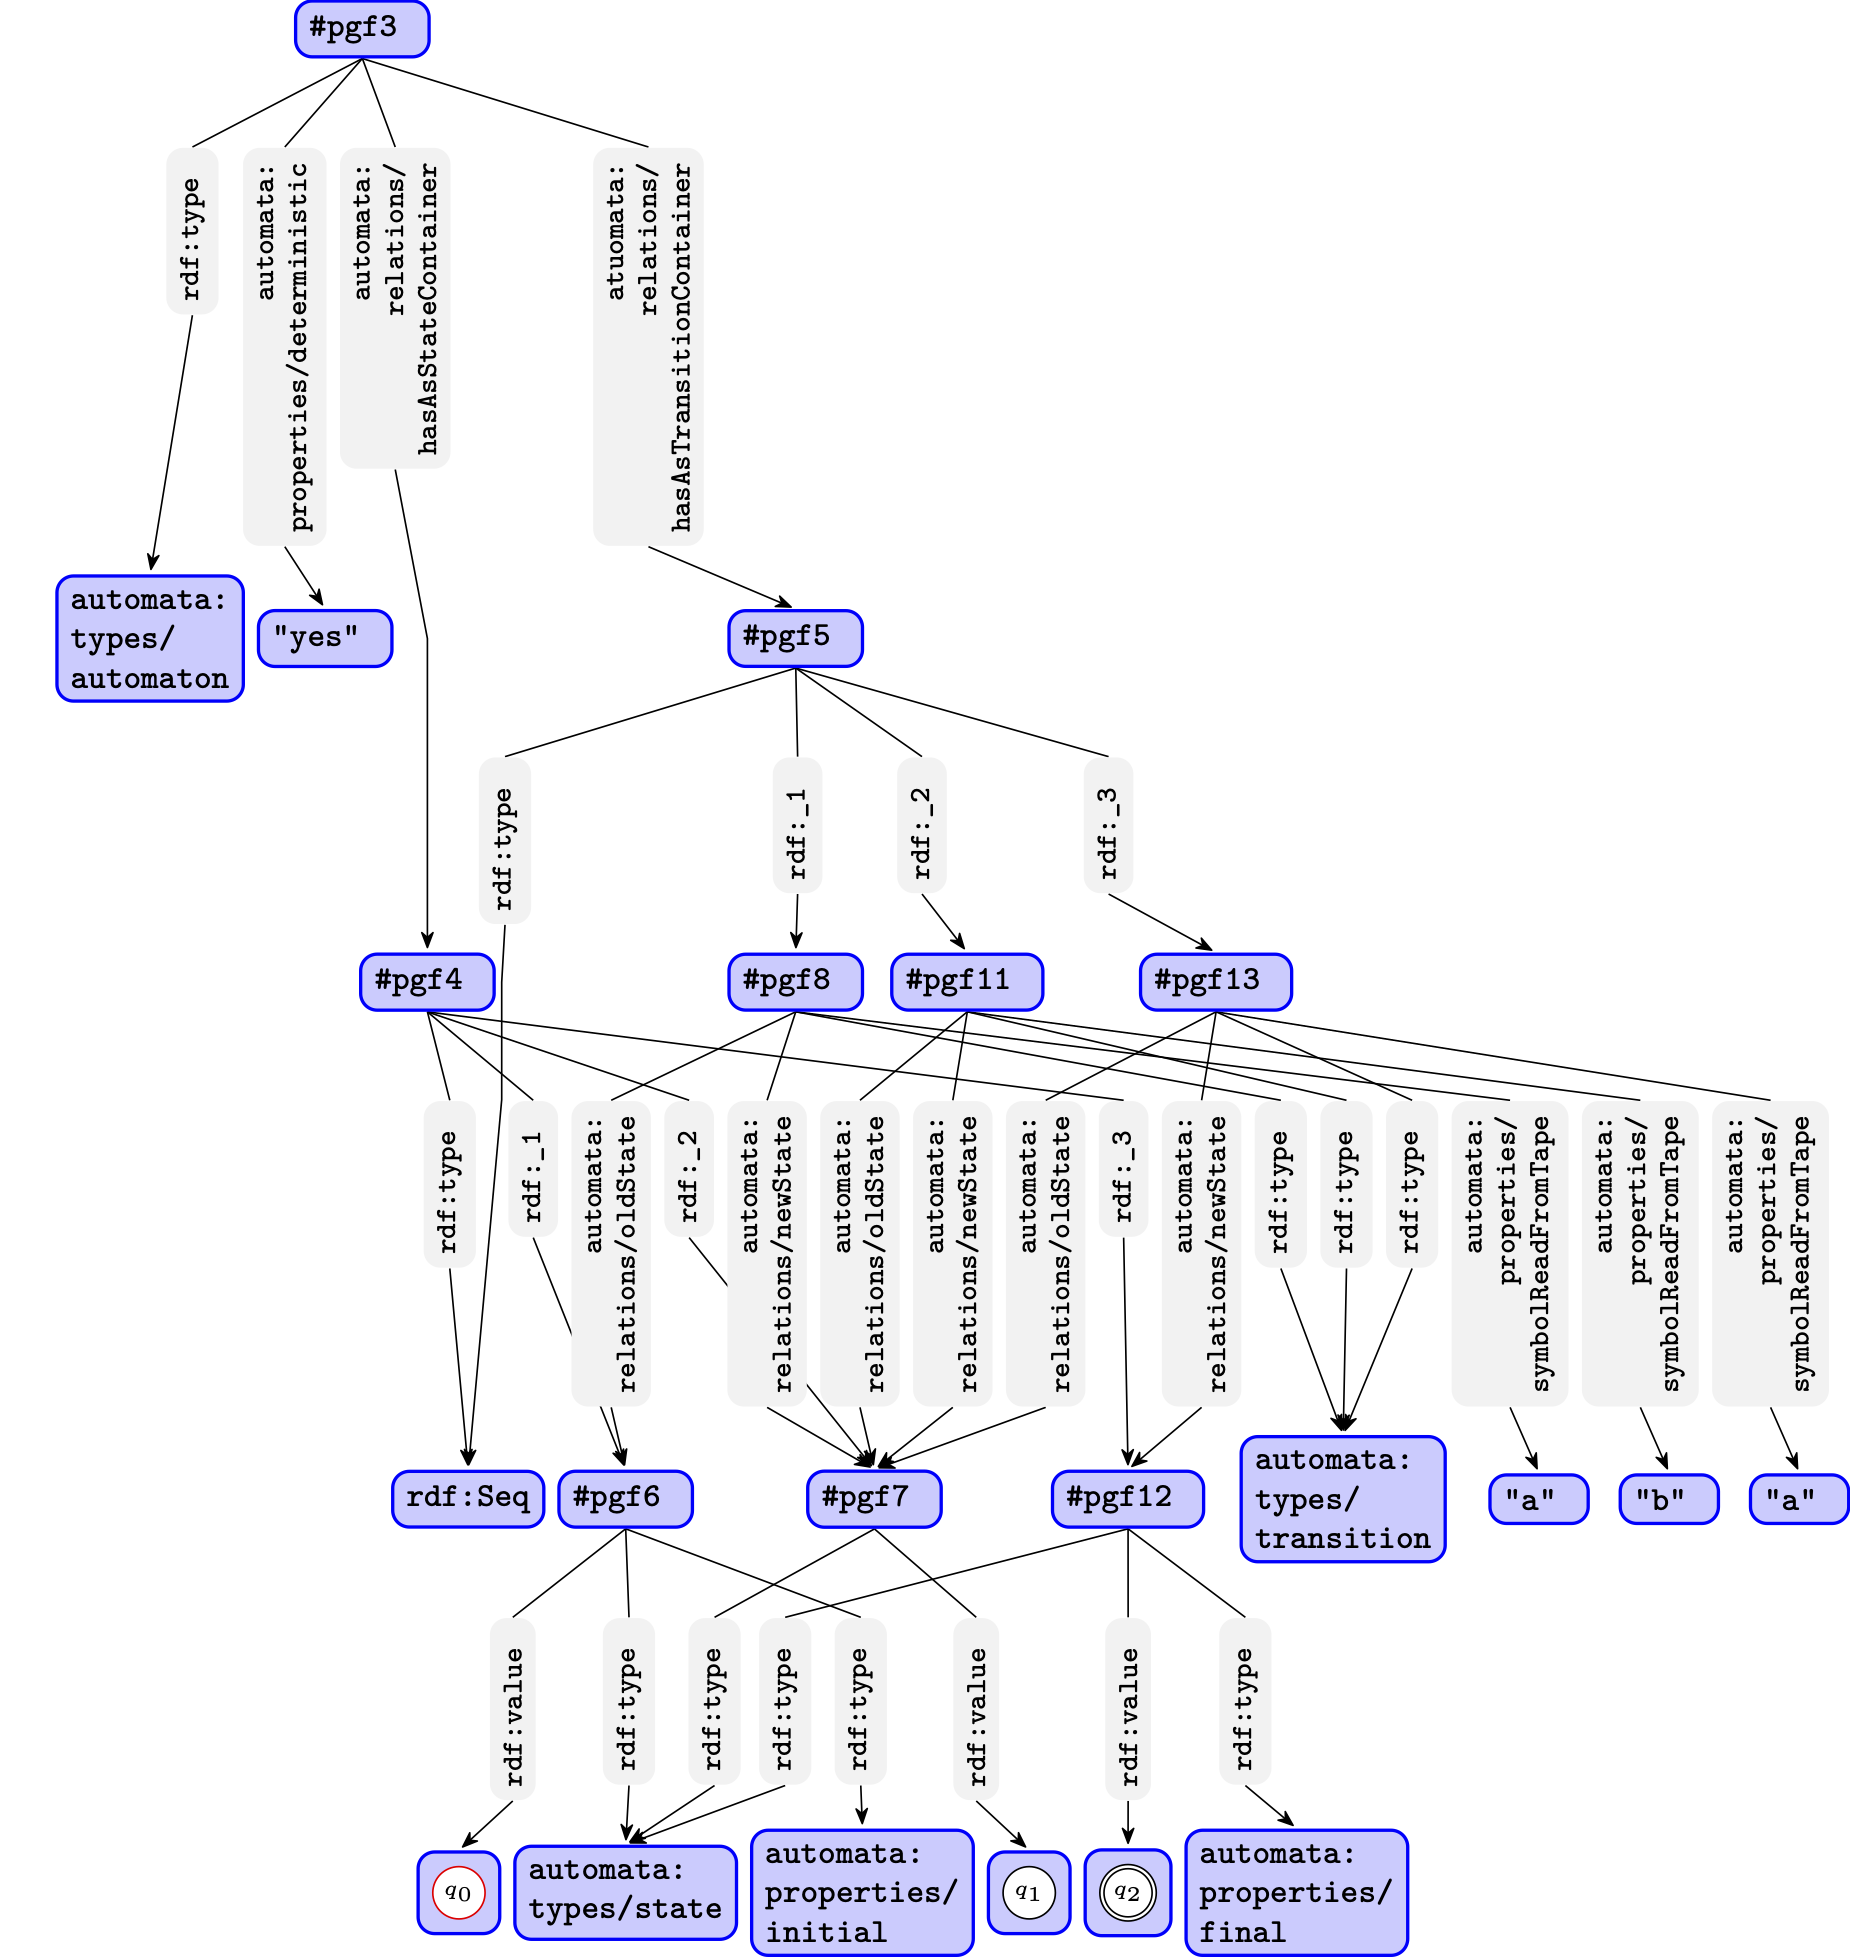
\includegraphics[width=\linewidth]{standalone/rdf.png}

\iffalse
\ifluatex
\else
    This example can only be typeset using Lua\TeX.
    \endgroup\expandafter\endinput
\fi

{
  % \newbox\myboxa
  % \setbox\myboxa=\hbox{\tiny {\tikz\node[circle, draw=red, fill=white] {$q_0$};}}
  % \newbox\myboxb
  % \setbox\myboxb=\hbox{\tiny {\tikz\node[circle, draw,fill=white] {$q_1$};}}
  % \newbox\myboxc
  % \setbox\myboxc=\hbox{\tiny {\tikz\node[circle, draw,fill=white, double] {$q_2$};}}
  \catcode`\_=11
  \begin{tikzpicture}[font=\tiny\ttfamily, > = {Stealth [round, sep]}]
  \graph [layered layout, sibling sep=1mm, sibling distance=0pt,
  resource/.style = {align=left,font=\footnotesize\ttfamily, draw = blue, thick, fill=blue!20, rounded corners},
  predicate/.style = {align=right,font=\scriptsize\ttfamily,fill=black!5,rotate=90,anchor=mid east, rounded corners},
  tail anchor=south, head anchor=north] {
    pgf3/\#pgf3[resource]   -- /"rdf:type"[predicate] -> automaton[as={automata:\\types/\\automaton},resource];
    pgf3/\#pgf3[resource]   -- /"automata:\\properties/deterministic"[predicate] -> /{"yes"}[resource];
    pgf4/\#pgf4[resource]   -- /"rdf:type"[predicate] -> rdf:Seq[resource];
    pgf3/\#pgf3[resource]   -- /"automata:\\relations/\\hasAsStateContainer"[predicate] -> pgf4[resource];
    pgf5/\#pgf5[resource]   -- /"rdf:type"[predicate] -> rdf:Seq[resource];
    pgf3/\#pgf3[resource]   -- /"atuomata:\\relations/\\hasAsTransitionContainer"[predicate] -> pgf5[resource];
    pgf6/\#pgf6[resource]   -- /"rdf:value"[predicate] -> /[as={\hbox{\tiny {\tikz\node[circle, draw=red, fill=white] {$q_0$};}}},resource];
    pgf6/\#pgf6[resource]   -- /"rdf:type"[predicate] -> state/"automata:\\types/state"[resource];
    pgf4/\#pgf4[resource]   -- /"rdf:_1"[predicate] -> pgf6[resource];
    pgf6/\#pgf6[resource]   -- /"rdf:type"[predicate] -> initial/"automata:\\properties/\\initial"[resource];
    pgf7/\#pgf7[resource]   -- /"rdf:value"[predicate] ->  /[as={\tiny {\tikz\node[circle, draw,fill=white] {$q_1$};}},resource];
    pgf7/\#pgf7[resource]   -- /"rdf:type"[predicate] -> state/"automata:\\types/state"[resource];
    pgf4/\#pgf4[resource]   -- /"rdf:_2"[predicate] -> pgf7[resource];
    pgf12/\#pgf12[resource] -- /"rdf:value"[predicate] -> /[as={\tiny {\tikz\node[circle, draw,fill=white, double] {$q_2$};}},resource];
    pgf12/\#pgf12[resource] -- /"rdf:type"[predicate] -> state/"automata:\\types/state"[resource];
    pgf4/\#pgf4[resource]   -- /"rdf:_3"[predicate] -> pgf12[resource];
    pgf12/\#pgf12[resource] -- /"rdf:type"[predicate] -> final/"automata:\\properties/\\final"[resource];
    pgf8/\#pgf8[resource]   -- /"rdf:type"[predicate] -> transition/"automata:\\types/\\transition"[resource];
    pgf8/\#pgf8[resource]   -- /"automata:\\properties/\\symbolReadFromTape"[predicate] -> /{"a"}[resource];
    pgf8/\#pgf8[resource]   -- /"automata:\\relations/oldState"[predicate] -> pgf6[resource];
    pgf8/\#pgf8[resource]   -- /"automata:\\relations/newState"[predicate] -> pgf7[resource];
    pgf5/\#pgf5[resource]   -- /"rdf:_1"[predicate] -> pgf8[resource];
    pgf11/\#pgf11[resource] -- /"rdf:type"[predicate] -> transition/"automata:\\types/\\transition"[resource];
    pgf11/\#pgf11[resource] -- /"automata:\\properties/\\symbolReadFromTape"[predicate] -> /{"b"}[resource];
    pgf11/\#pgf11[resource] -- /"automata:\\relations/oldState"[predicate] -> pgf7[resource];
    pgf11/\#pgf11[resource] -- /"automata:\\relations/newState"[predicate] -> pgf7[resource];
    pgf5/\#pgf5[resource]   -- /"rdf:_2"[predicate] -> pgf11[resource];
    pgf13/\#pgf13[resource] -- /"rdf:type"[predicate] -> transition/"automata:\\types/\\transition"[resource];
    pgf13/\#pgf13[resource] -- /"automata:\\properties/\\symbolReadFromTape"[predicate] -> /{"a"}[resource];
    pgf13/\#pgf13[resource] -- /"automata:\\relations/oldState"[predicate] -> pgf7[resource];
    pgf13/\#pgf13[resource] -- /"automata:\\relations/newState"[predicate] -> pgf12[resource];
    pgf5/\#pgf5[resource]   -- /"rdf:_3"[predicate] -> pgf13[resource];
  };
\end{tikzpicture}
}

\endgroup
\fi